 \documentclass{beamer}

\usetheme{MagdeburgFIN}
\usefonttheme{structurebold}
\usepackage{graphicx}
\usepackage{float}
\usepackage{url}
\usepackage{pdfpages}


\title{SIMD Acceleration for Index Structures}
\author{Marten Wallewein-Eising}
\date{\today}
\institute{Otto von Guericke Univerity, Magdeburg}

\begin{document}

\begin{frame}[plain]
 \titlepage
\end{frame}



\section[Agenda]{}
\begin{frame}
\frametitle{Agenda}
\tableofcontents
\end{frame}

\section{Motivation}
\begin{frame}
\frametitle{Motivation}
	\begin{center}
		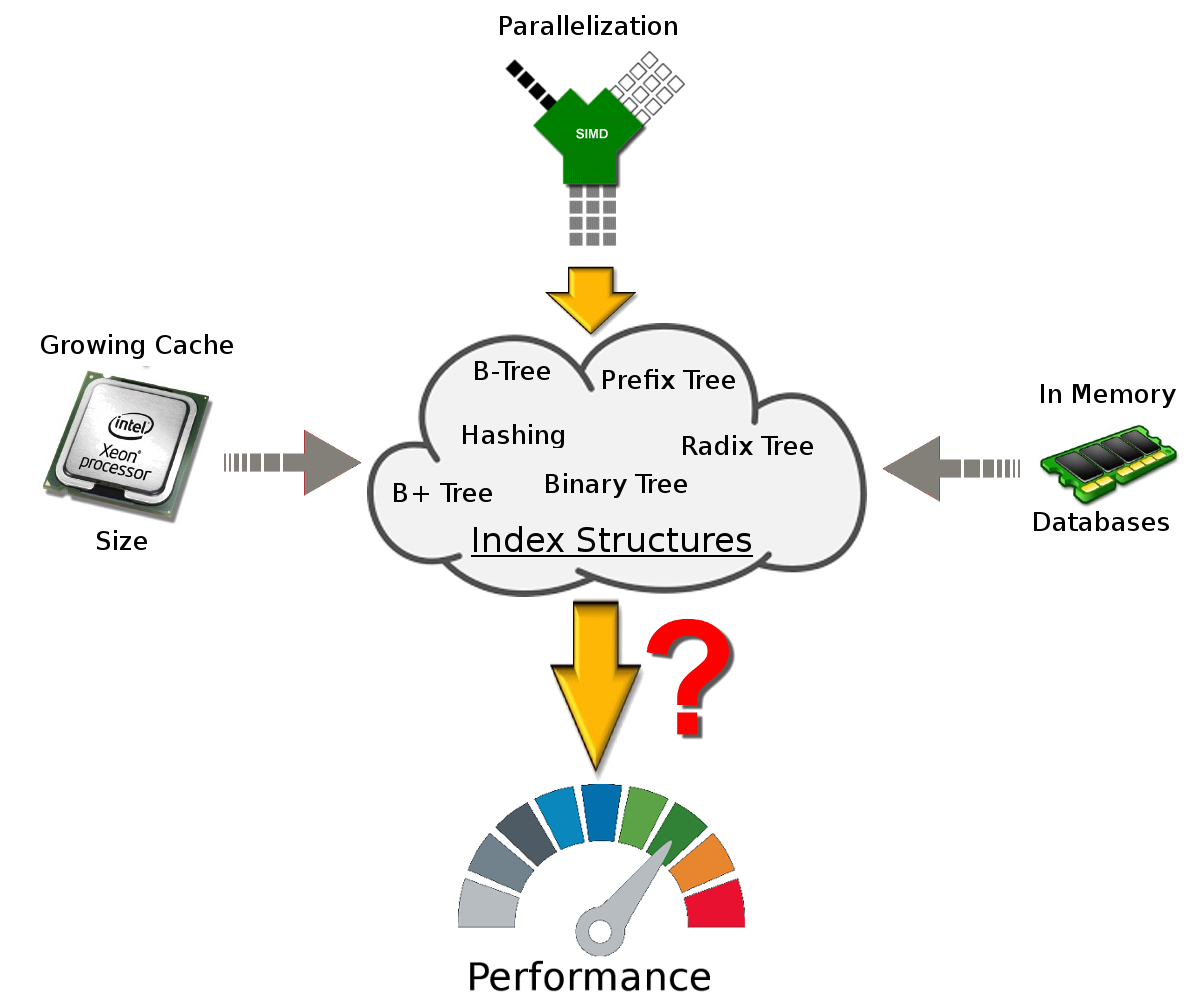
\includegraphics[width=0.7\textwidth]{img/big_picture.png}
	\end{center}
\end{frame}

%\section{B$^{+}$- and Radix-Trees}
\section{Excursion: B$^{+}$-Tree} 
\begin{frame}
\frametitle{Excursion: B$^{+}$-Tree}
\begin{center}
	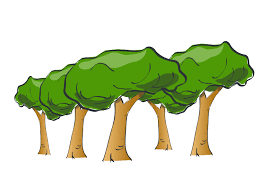
\includegraphics[width=0.5\textwidth]{img/forest.png}
\end{center}
\end{frame}
\begin{frame}
\frametitle{B$^{+}$-Tree}
	\begin{center}
		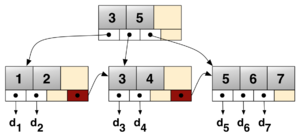
\includegraphics[width=0.6\textwidth]{img/bplus_tree.png}
	\end{center}
	\begin{itemize}
		\item N-ary tree with often a large number of children per node
		\item Only leaf nodes contain keys
		\item Leaf nodes often linked for range based scans
	\end{itemize}
\end{frame}
%\begin{frame}
%\frametitle{Radix-Tree}
%	\begin{center}
%	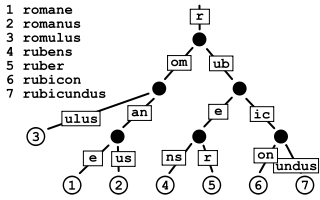
\includegraphics[width=0.6\textwidth]{img/radix_tree.png}
%	\end{center}
%	\begin{itemize}
%		\item Space optimized prefix tree
%		\item Number of children of every inner node is at least the radix $r$
%		\item Each node that is the only child is merged with its parent
%	\end{itemize}
%\end{frame}
\section{SIMD Style Processing}
\begin{frame}
\frametitle{Single Instruction Multiple Data}
\begin{center}
	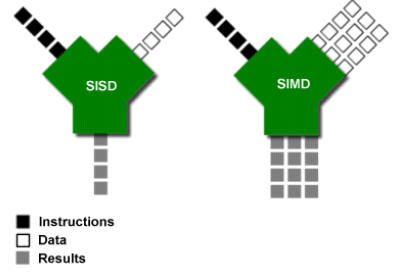
\includegraphics[width=0.6\textwidth]{img/simd.png}
\end{center}
\begin{itemize}
	\item \textbf{\_\_m128i \_mm\_cmpgt\_epi32 (\_\_m128i a, \_\_m128i b)} Compares 4 signed 32-bit integers in a and 4 signed 32-bit integers
	in b for greater-than.
\end{itemize}
\end{frame}
%\begin{frame}
%\frametitle{Horizontal Vectorization}
%\begin{center}
%	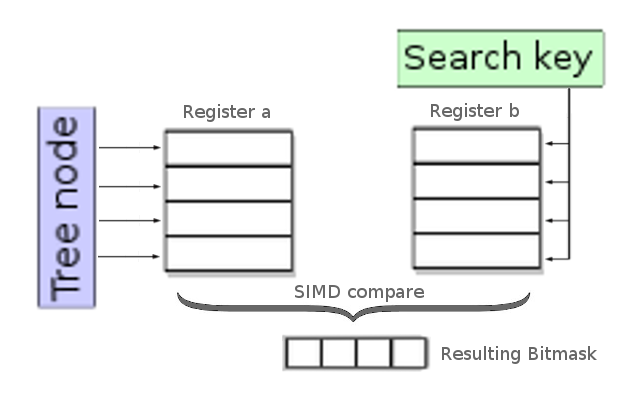
\includegraphics[width=0.6\textwidth]{img/horizontal_vectorization.png}
%\end{center}
%\begin{itemize}
%	\item Compare one search key to multiple keys of the index structure
%	\item Opposite: Vertical vectorization
%	\begin{itemize}
%		\item Not possible, since sequential data storage in main memory is needed
%	\end{itemize}
%\end{itemize}
%\end{frame}
\section{Adapted Tree structures}

\begin{frame}
\frametitle{Adapted Index Structures}
\begin{itemize}
	\item Seg-Tree/Trie
	\item FAST: Fast Architecture Sensitive Tree
	\item VAST: Vector-Advanced and Compressed Structure Tree
	\item ART: Adaptive Radix Tree
\end{itemize}
\end{frame}

\subsection{Seg-Tree/Trie}
\begin{frame}
\frametitle{Seg-Tree/Trie}
\begin{center}
	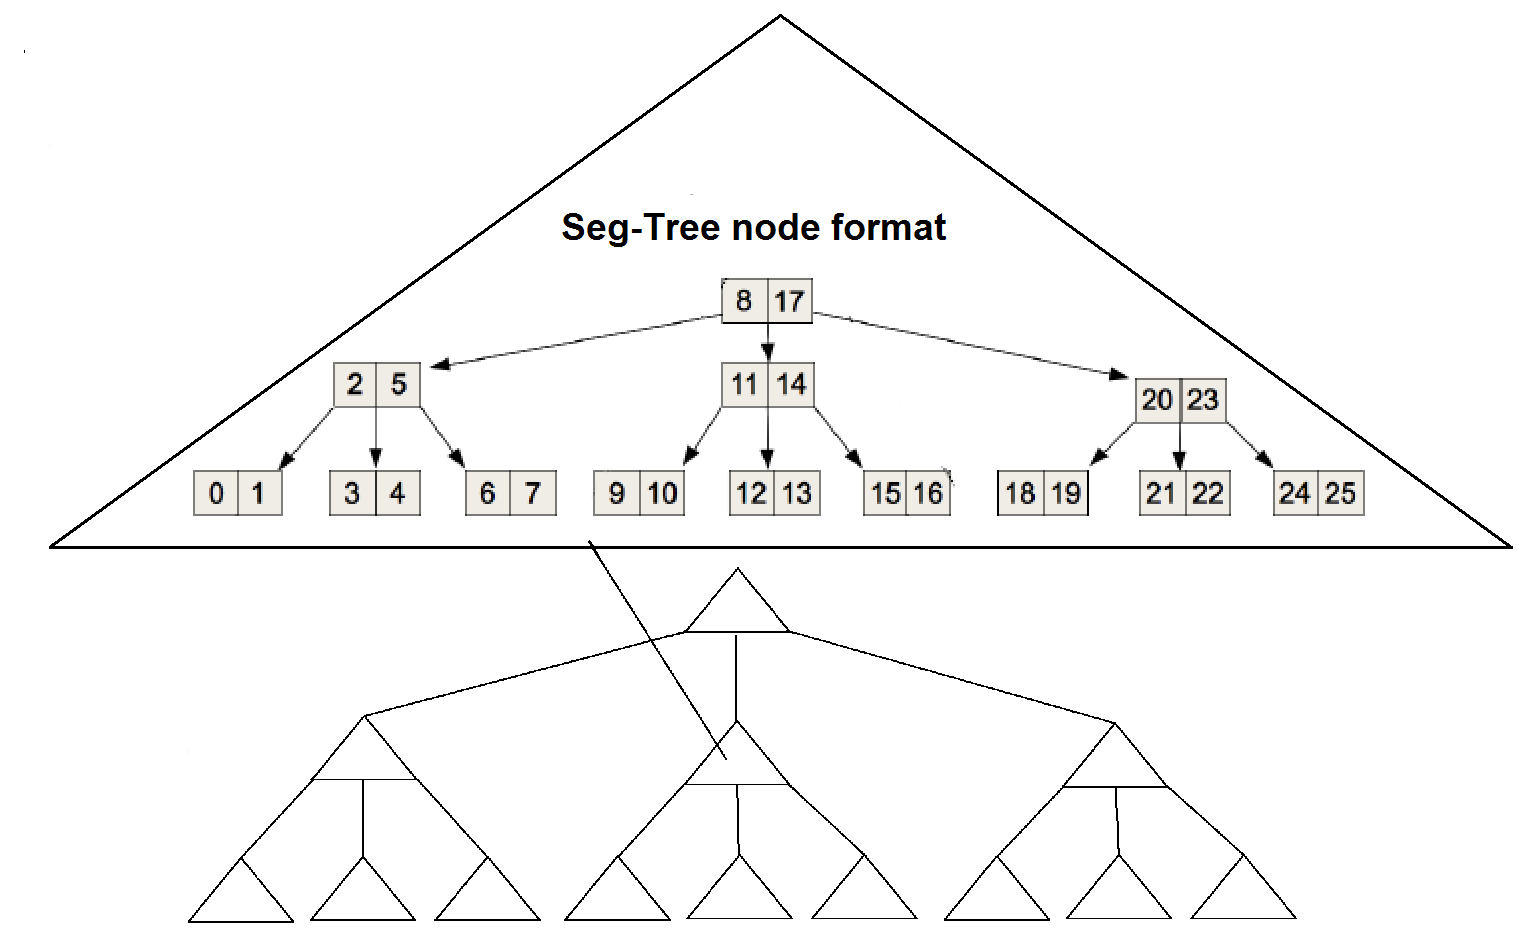
\includegraphics[width=0.7\textwidth]{img/seg_tree2.png}
\end{center}
\begin{itemize}
	\item Each node is a k-ary search tree
	\item Each node is linearised to use k-ary search
	\item $k = \frac{\vert SIMD \vert }{\vert Key \vert}$, k keys are compared in parallel
	%\item Each node is a k-ary search tree
\end{itemize}
\end{frame}
\subsection{FAST}
\begin{frame}
\frametitle{Fast Architecture Sensitive Tree}
\begin{center}
	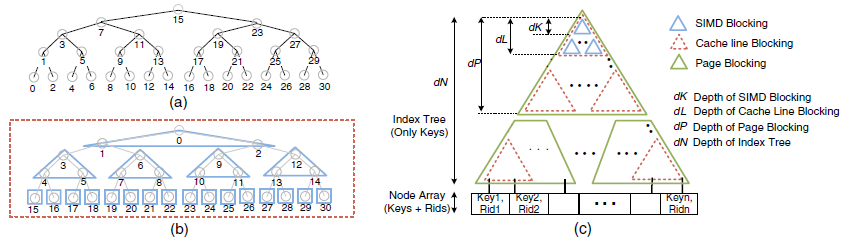
\includegraphics[width=1.05\textwidth]{img/fast.png}
\end{center}
\begin{itemize}
	\item Based on binary tree
	\item Hierarchical blocking: SIMD, cache line and page blocks
	\item Efficient cache line and page usage
\end{itemize}
\end{frame}
\begin{frame}
\frametitle{Adapted Index Structures}
\begin{itemize}
	\item VAST: Vector-Advanced and Compressed Structure Tree
	\begin{itemize}
		\item Extension of FAST
		\item Uses key compression on lower levels of the tree
	\end{itemize}
	\item ART: Adaptive Radix Tree
	\begin{itemize}
		\item Uses different node types with different number of keys and children
		\item Due to overfill or underfill of nodes, the node type is changed
	\end{itemize}
\end{itemize}
\end{frame}
\subsection{VAST}
%\begin{frame}
%\frametitle{Vector-Advanced and Compressed Structure Tree}
%\begin{center}
%	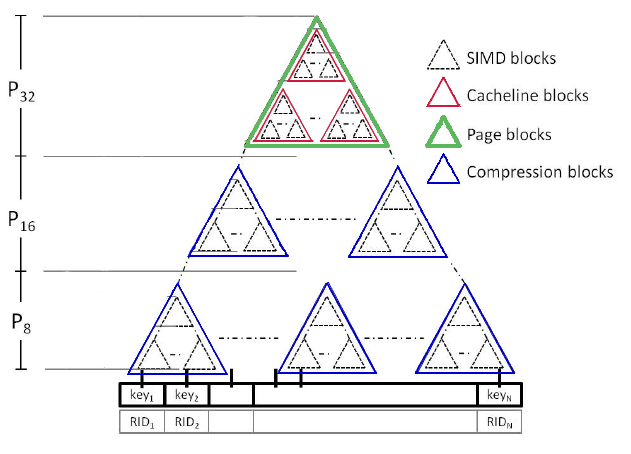
\includegraphics[width=0.5\textwidth]{img/vast2.png}
%\end{center}
%	\begin{itemize}
%	\item Layer $P_{32}$ same blocking structure as FAST, 32 Bit keys
%	\item Layer $P_{16}$ and $P_{8}$ compressed keys to 16 and 8 Bit (lossy)
%	\item Leaf nodes compressed lossless
%\end{itemize}
%\end{frame}
\subsection{ART}
%\begin{frame}
%\frametitle{Adaptive Radix Tree}
%\begin{center}
%	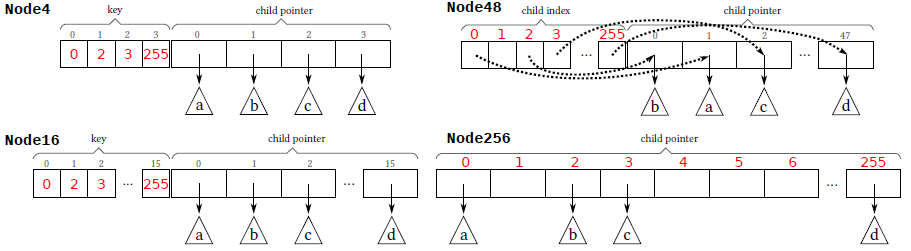
\includegraphics[width=1.05\textwidth]{img/art2.png}
%\end{center}
%\begin{itemize}
%	\item Different node formats and sizes
%	\begin{itemize}
%		\item More flexible
%	\end{itemize}
%	\item Horizontal Vectorization on keys of \emph{Node16}
%	\item Lazy expansion and path compression
%\end{itemize}
%\end{frame}
\section{Evaluation}

%\begin{frame}
%\frametitle{Evaluation}
%Important criteria for performance increase:
%\begin{itemize}
%	\item Horizontal vectorization
%	\item Minimized key size
%	\item Adapted node sizes and types
%	\item Decreased branch misses
%	\item Full use of cache line using blocking and alignment
%	\item Usage of compression
%	\item Adapt search algorithm for linearised nodes
%\end{itemize}
%\end{frame}

\begin{frame}
\frametitle{Evaluation}
Implementation of the considered performance criteria and their impact:
\begin{figure}
	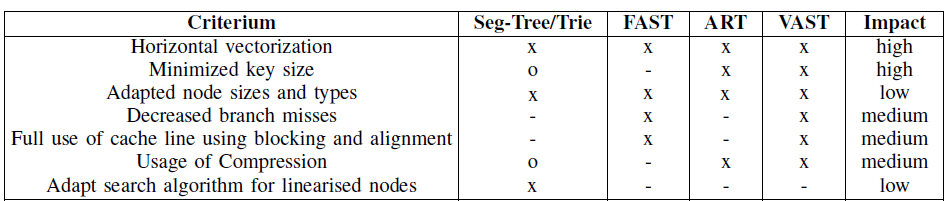
\includegraphics[width=1.05\textwidth]{img/table_eval.png}
\end{figure}
Legend: x: implements the issue, o: partially implements the issue, -: not implements the issue
\end{frame}

\section{Conclusion}
\begin{frame}
\frametitle{Conclusion}
How to adapt index structures to modern database systems:
\begin{itemize}
	\item Compare as many keys as possible in parallel with SIMD
	\begin{itemize}
		\item Direct performance increase up to a multiple
	\end{itemize}
	\item Efficient usage of cache line
	\item Decrease branch misses
	\item Use compression or adapted search algorithms
	\end{itemize}
\end{frame}

\begin{frame}
\frametitle{Sources}
\begin{itemize}
	\item \url{http://infolab.stanford.edu/~nsample/cs245/handouts/hw2sol/sol2.html}
	%\item \url{https://en.wikipedia.org/wiki/Radix\_tree}
	\item \url{https://www.clker.com/clipart-bosque.html}
	\item S. Zeuch, F. Huber and J.-C. Freytag  ``Adapting Tree Structures for Processing with SIMD Instructions'' in EDBT, 2014.
	\item C. Kim, J. Chhugani, N. Satish, E. Sedlar, A. D. Nguyen, T. Kaldewey, V. W. Lee, S. A. Brandt and P. Dubey ``FAST: Fast Architecture Sensitive Tree Search on Modern CPUs and GPUs'' in SIGMOD, pp. 339-350, 2010.
	\item V. Leis, A. Kemper and T. Neumann ``The Adaptive Radix Tree: ARTful Indexing for Main-Memory Databases'' in ICDE, pages 38-49, 2013.
\end{itemize}
\end{frame}

\begin{frame}
\frametitle{Sources}
\begin{itemize}
	\item T. Yamamuro, M. Onizuka, T. Hitaka, and M. Yamamuro ``VAST-Tree: A Vector-Advanced and Compressed Structure for Massive Data Tree Traversal'' in EDBT, pp. 396-407, 2012.
\end{itemize}
\end{frame}

\begin{frame}
 \frametitle{Thank you for your attention!}
\end{frame}
\end{document}
